\section{实验:研究杠杆的平衡条件}\label{sec:7-2}

\shiyan{目的} 研究杠杆在什么条件下平衡\footnote{杠杆静止不转或者匀速转动都叫做杠杆平衡。}。

\shiyan{器材} 杠杆和它的支架,弹簧秤,钩码,尺,线。

\shiyan{步骤}

(1) 把杠杆的中点支在支架上,调节杠杆两端的螺母,使杠杆在水平位置平衡。

(2) 照图 \ref{fig:7-3} 那样,把钩码挂在杠杆两边,改变钩码的位置,仍使杠杆在水平位置平衡。

我们把支点左方的钩码作用于杠杆的力(等于钩码重)当作阻力,
把支点右方的钩码作用于杠杆的力当作动力。
将动力 $F_1$、阻力 $F_2$、动力臂 $l_1$、阻力臂 $l_2$ 的数值填入下表。

\begin{figure}[htbp]
    \centering
    \begin{minipage}{7cm}
    \centering
    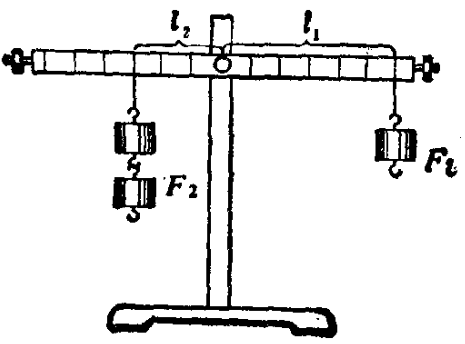
\includegraphics[width=7cm]{../pic/czwl1-ch7-3}
    \caption{}\label{fig:7-3}
    \end{minipage}
    \qquad
    \begin{minipage}{7cm}
    \centering
    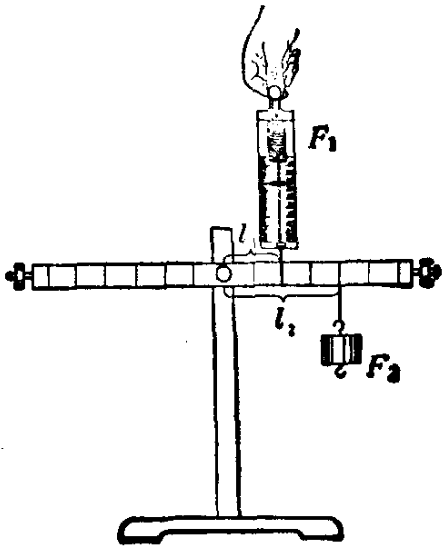
\includegraphics[width=6cm]{../pic/czwl1-ch7-4}
    \caption{}\label{fig:7-4}
    \end{minipage}
\end{figure}

(3) 改变力和力臂的数值,再做三次实验,将结果填入下表。

\begin{table}[H]
    \centering
    %\begin{tabular}{|w{c}{4em}|*{2}{w{c}{4em}|}w{c}{6em}|*{2}{w{c}{4em}|}w{c}{6em}|}
    \begin{tabular}{|w{c}{4em}|*{2}{*{2}{w{c}{4em}|}w{c}{6em}|}}
        \hline
        \tabincell{c}{实验\\次数} & \tabincell{c}{动力\\($F_1$)\\(牛顿)} & \tabincell{c}{动力臂\\($l_1$)\\(厘米)} & \tabincell{c}{动力 $\times$ 动力臂\\ $F_1 \cdot l_1$} & \tabincell{c}{阻力\\($F_2$)\\(牛顿)} & \tabincell{c}{阻力臂\\($l_2$)\\(厘米)} & \tabincell{c}{阻力 $\times$ 阻力臂\\$F_2 \cdot l_2$} \\ \hline
        1 & & & & & & \\ \hline
        2 & & & & & & \\ \hline
        3 & & & & & & \\ \hline
        4 & & & & & & \\ \hline
    \end{tabular}
\end{table}

(4) 求出各次实验中动力 $\times$ 动力臂和阻力 $\times$ 阻力臂的数值。
根据得到的结果研究杠杆在什么条件下平衡。

(5) 仿照上表自己再绘制一张表。

(6) 照图 \ref{fig:7-4} 那样,把钩码挂在杠杆上,用弹簧秤拉着杠杆,使杠杆在水平位置平衡。
把钩码作用于杠杆的力当作阻力 $F_2$,弹簧秤的拉力当作动力 $F_1$。
改变力和力臂的数值再做三次实验。将四次实验的结果填入自己画的表内,
根据实验结果研究杠杆在什么条件下平衡。

